\documentclass[twoside]{book}

% Packages required by doxygen
\usepackage{fixltx2e}
\usepackage{calc}
\usepackage{doxygen}
\usepackage[export]{adjustbox} % also loads graphicx
\usepackage{graphicx}
\usepackage[utf8]{inputenc}
\usepackage{makeidx}
\usepackage{multicol}
\usepackage{multirow}
\PassOptionsToPackage{warn}{textcomp}
\usepackage{textcomp}
\usepackage[nointegrals]{wasysym}
\usepackage[table]{xcolor}

% Font selection
\usepackage[T1]{fontenc}
\usepackage[scaled=.90]{helvet}
\usepackage{courier}
\usepackage{amssymb}
\usepackage{sectsty}
\renewcommand{\familydefault}{\sfdefault}
\allsectionsfont{%
  \fontseries{bc}\selectfont%
  \color{darkgray}%
}
\renewcommand{\DoxyLabelFont}{%
  \fontseries{bc}\selectfont%
  \color{darkgray}%
}
\newcommand{\+}{\discretionary{\mbox{\scriptsize$\hookleftarrow$}}{}{}}

% Page & text layout
\usepackage{geometry}
\geometry{%
  a4paper,%
  top=2.5cm,%
  bottom=2.5cm,%
  left=2.5cm,%
  right=2.5cm%
}
\tolerance=750
\hfuzz=15pt
\hbadness=750
\setlength{\emergencystretch}{15pt}
\setlength{\parindent}{0cm}
\setlength{\parskip}{3ex plus 2ex minus 2ex}
\makeatletter
\renewcommand{\paragraph}{%
  \@startsection{paragraph}{4}{0ex}{-1.0ex}{1.0ex}{%
    \normalfont\normalsize\bfseries\SS@parafont%
  }%
}
\renewcommand{\subparagraph}{%
  \@startsection{subparagraph}{5}{0ex}{-1.0ex}{1.0ex}{%
    \normalfont\normalsize\bfseries\SS@subparafont%
  }%
}
\makeatother

% Headers & footers
\usepackage{fancyhdr}
\pagestyle{fancyplain}
\fancyhead[LE]{\fancyplain{}{\bfseries\thepage}}
\fancyhead[CE]{\fancyplain{}{}}
\fancyhead[RE]{\fancyplain{}{\bfseries\leftmark}}
\fancyhead[LO]{\fancyplain{}{\bfseries\rightmark}}
\fancyhead[CO]{\fancyplain{}{}}
\fancyhead[RO]{\fancyplain{}{\bfseries\thepage}}
\fancyfoot[LE]{\fancyplain{}{}}
\fancyfoot[CE]{\fancyplain{}{}}
\fancyfoot[RE]{\fancyplain{}{\bfseries\scriptsize Generated by Doxygen }}
\fancyfoot[LO]{\fancyplain{}{\bfseries\scriptsize Generated by Doxygen }}
\fancyfoot[CO]{\fancyplain{}{}}
\fancyfoot[RO]{\fancyplain{}{}}
\renewcommand{\footrulewidth}{0.4pt}
\renewcommand{\chaptermark}[1]{%
  \markboth{#1}{}%
}
\renewcommand{\sectionmark}[1]{%
  \markright{\thesection\ #1}%
}

% Indices & bibliography
\usepackage{natbib}
\usepackage[titles]{tocloft}
\setcounter{tocdepth}{3}
\setcounter{secnumdepth}{5}
\makeindex

% Hyperlinks (required, but should be loaded last)
\usepackage{ifpdf}
\ifpdf
  \usepackage[pdftex,pagebackref=true]{hyperref}
\else
  \usepackage[ps2pdf,pagebackref=true]{hyperref}
\fi
\hypersetup{%
  colorlinks=true,%
  linkcolor=blue,%
  citecolor=blue,%
  unicode%
}

% Custom commands
\newcommand{\clearemptydoublepage}{%
  \newpage{\pagestyle{empty}\cleardoublepage}%
}

\usepackage{caption}
\captionsetup{labelsep=space,justification=centering,font={bf},singlelinecheck=off,skip=4pt,position=top}

%===== C O N T E N T S =====

\begin{document}

% Titlepage & ToC
\hypersetup{pageanchor=false,
             bookmarksnumbered=true,
             pdfencoding=unicode
            }
\pagenumbering{alph}
\begin{titlepage}
\vspace*{7cm}
\begin{center}%
{\Large Geometria en python \\[1ex]\large 1.\+0 }\\
\vspace*{1cm}
{\large Generated by Doxygen 1.8.13}\\
\end{center}
\end{titlepage}
\clearemptydoublepage
\pagenumbering{roman}
\tableofcontents
\clearemptydoublepage
\pagenumbering{arabic}
\hypersetup{pageanchor=true}

%--- Begin generated contents ---
\chapter{Hierarchical Index}
\section{Class Hierarchy}
This inheritance list is sorted roughly, but not completely, alphabetically\+:\begin{DoxyCompactList}
\item \contentsline{section}{Imports.\+Impresora.\+Impresora}{\pageref{class_imports_1_1_impresora_1_1_impresora}}{}
\item \contentsline{section}{Imports.\+Principal.\+Principal}{\pageref{class_imports_1_1_principal_1_1_principal}}{}
\item \contentsline{section}{Imports.\+Vertice.\+Vertice}{\pageref{class_imports_1_1_vertice_1_1_vertice}}{}
\begin{DoxyCompactList}
\item \contentsline{section}{Imports.\+Figura.\+Figura}{\pageref{class_imports_1_1_figura_1_1_figura}}{}
\begin{DoxyCompactList}
\item \contentsline{section}{Imports.\+Circulo.\+Circulo}{\pageref{class_imports_1_1_circulo_1_1_circulo}}{}
\item \contentsline{section}{Imports.\+Rectangulo.\+Rectangulo}{\pageref{class_imports_1_1_rectangulo_1_1_rectangulo}}{}
\item \contentsline{section}{Imports.\+Triangulo.\+Triangulo}{\pageref{class_imports_1_1_triangulo_1_1_triangulo}}{}
\begin{DoxyCompactList}
\item \contentsline{section}{Imports.\+Triangulo.\+Equilatero}{\pageref{class_imports_1_1_triangulo_1_1_equilatero}}{}
\item \contentsline{section}{Imports.\+Triangulo.\+Escaleno}{\pageref{class_imports_1_1_triangulo_1_1_escaleno}}{}
\item \contentsline{section}{Imports.\+Triangulo.\+Isosceles}{\pageref{class_imports_1_1_triangulo_1_1_isosceles}}{}
\end{DoxyCompactList}
\end{DoxyCompactList}
\end{DoxyCompactList}
\end{DoxyCompactList}

\chapter{Class Index}
\section{Class List}
Here are the classes, structs, unions and interfaces with brief descriptions\+:\begin{DoxyCompactList}
\item\contentsline{section}{\hyperlink{class_binary_search_tree}{Binary\+Search\+Tree$<$ Data, Type\+Nodo $>$} }{\pageref{class_binary_search_tree}}{}
\item\contentsline{section}{\hyperlink{class_circulo}{Circulo} \\*Clase que se encarga e modelar un circulo }{\pageref{class_circulo}}{}
\item\contentsline{section}{\hyperlink{class_class_node}{Class\+Node$<$ Dato $>$} }{\pageref{class_class_node}}{}
\item\contentsline{section}{\hyperlink{class_dato_no_primitivo}{Dato\+No\+Primitivo$<$ Tipo\+Dato $>$} }{\pageref{class_dato_no_primitivo}}{}
\item\contentsline{section}{\hyperlink{class_equilatero}{Equilatero} \\*Calse equilatero }{\pageref{class_equilatero}}{}
\item\contentsline{section}{\hyperlink{class_escaleno}{Escaleno} \\*Calse \hyperlink{class_escaleno}{Escaleno} }{\pageref{class_escaleno}}{}
\item\contentsline{section}{\hyperlink{class_figura}{Figura} \\*Clase que se encarga de crear una figura en 2D }{\pageref{class_figura}}{}
\item\contentsline{section}{\hyperlink{class_impresora}{Impresora$<$ T $>$} \\*Clase que imprmime objetos }{\pageref{class_impresora}}{}
\item\contentsline{section}{\hyperlink{class_isosceles}{Isosceles} \\*Calse \hyperlink{class_isosceles}{Isosceles} }{\pageref{class_isosceles}}{}
\item\contentsline{section}{\hyperlink{class_principal}{Principal} }{\pageref{class_principal}}{}
\item\contentsline{section}{\hyperlink{classrectangulo}{rectangulo} \\*Clase rectangulo }{\pageref{classrectangulo}}{}
\item\contentsline{section}{\hyperlink{classtriangulo}{triangulo} \\*Calse tringulo }{\pageref{classtriangulo}}{}
\item\contentsline{section}{\hyperlink{class_vertice}{Vertice} \\*Clase que modela un punto en el espacio }{\pageref{class_vertice}}{}
\end{DoxyCompactList}

\chapter{Class Documentation}
\hypertarget{class_imports_1_1_circulo_1_1_circulo}{}\section{Imports.\+Circulo.\+Circulo Class Reference}
\label{class_imports_1_1_circulo_1_1_circulo}\index{Imports.\+Circulo.\+Circulo@{Imports.\+Circulo.\+Circulo}}


Inheritance diagram for Imports.\+Circulo.\+Circulo\+:
\nopagebreak
\begin{figure}[H]
\begin{center}
\leavevmode
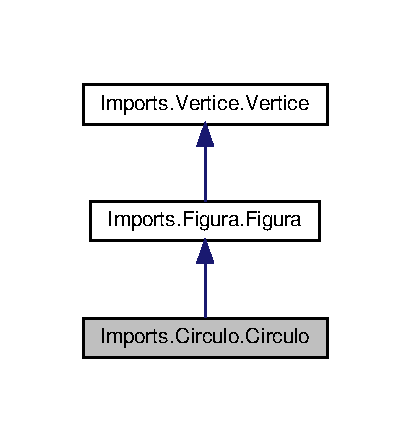
\includegraphics[width=197pt]{class_imports_1_1_circulo_1_1_circulo__inherit__graph}
\end{center}
\end{figure}


Collaboration diagram for Imports.\+Circulo.\+Circulo\+:
\nopagebreak
\begin{figure}[H]
\begin{center}
\leavevmode
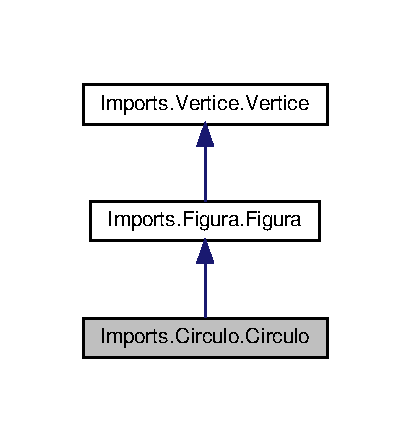
\includegraphics[width=197pt]{class_imports_1_1_circulo_1_1_circulo__coll__graph}
\end{center}
\end{figure}
\subsection*{Public Member Functions}
\begin{DoxyCompactItemize}
\item 
\mbox{\Hypertarget{class_imports_1_1_circulo_1_1_circulo_a90287ae374f2d878fe06eb7216a8d8f1}\label{class_imports_1_1_circulo_1_1_circulo_a90287ae374f2d878fe06eb7216a8d8f1}} 
def {\bfseries \+\_\+\+\_\+init\+\_\+\+\_\+} (self, arreglo\+Vertices)
\item 
\mbox{\Hypertarget{class_imports_1_1_circulo_1_1_circulo_adea3a7929a35ba35da26bf85ccc1cf8f}\label{class_imports_1_1_circulo_1_1_circulo_adea3a7929a35ba35da26bf85ccc1cf8f}} 
def {\bfseries superficie} (self)
\item 
\mbox{\Hypertarget{class_imports_1_1_circulo_1_1_circulo_ac6de431753ff0ad18300c9d40c2b770e}\label{class_imports_1_1_circulo_1_1_circulo_ac6de431753ff0ad18300c9d40c2b770e}} 
def {\bfseries perimetro} (self)
\end{DoxyCompactItemize}
\subsection*{Public Attributes}
\begin{DoxyCompactItemize}
\item 
\mbox{\Hypertarget{class_imports_1_1_circulo_1_1_circulo_a175156b15659fcd292d8fbe58fdf969b}\label{class_imports_1_1_circulo_1_1_circulo_a175156b15659fcd292d8fbe58fdf969b}} 
{\bfseries cantidad\+Puntos}
\item 
\mbox{\Hypertarget{class_imports_1_1_circulo_1_1_circulo_a46cb935cbe3cc97bc12f1a1ebf550245}\label{class_imports_1_1_circulo_1_1_circulo_a46cb935cbe3cc97bc12f1a1ebf550245}} 
{\bfseries lista\+Vertices}
\item 
\mbox{\Hypertarget{class_imports_1_1_circulo_1_1_circulo_ae475f236c5ad145218abda4272137fef}\label{class_imports_1_1_circulo_1_1_circulo_ae475f236c5ad145218abda4272137fef}} 
{\bfseries radio}
\item 
\mbox{\Hypertarget{class_imports_1_1_circulo_1_1_circulo_a5073418c67dc687d23ec5aadb638ae33}\label{class_imports_1_1_circulo_1_1_circulo_a5073418c67dc687d23ec5aadb638ae33}} 
{\bfseries para\+Imprimir}
\item 
\mbox{\Hypertarget{class_imports_1_1_circulo_1_1_circulo_a1dfc20a0297e0f52ab8e9e6da90af79b}\label{class_imports_1_1_circulo_1_1_circulo_a1dfc20a0297e0f52ab8e9e6da90af79b}} 
{\bfseries area}
\item 
\mbox{\Hypertarget{class_imports_1_1_circulo_1_1_circulo_a44f63cbe287165b871274309cbb85c98}\label{class_imports_1_1_circulo_1_1_circulo_a44f63cbe287165b871274309cbb85c98}} 
{\bfseries perimetrofig}
\end{DoxyCompactItemize}


The documentation for this class was generated from the following file\+:\begin{DoxyCompactItemize}
\item 
sourcecode/\+Imports/Circulo.\+py\end{DoxyCompactItemize}

\hypertarget{class_imports_1_1_triangulo_1_1_equilatero}{}\section{Imports.\+Triangulo.\+Equilatero Class Reference}
\label{class_imports_1_1_triangulo_1_1_equilatero}\index{Imports.\+Triangulo.\+Equilatero@{Imports.\+Triangulo.\+Equilatero}}


Inheritance diagram for Imports.\+Triangulo.\+Equilatero\+:
\nopagebreak
\begin{figure}[H]
\begin{center}
\leavevmode
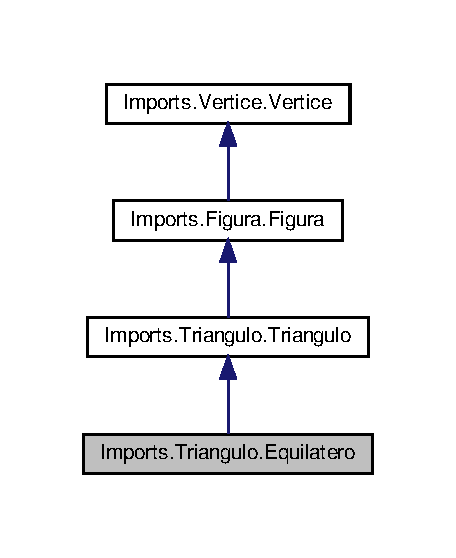
\includegraphics[width=219pt]{class_imports_1_1_triangulo_1_1_equilatero__inherit__graph}
\end{center}
\end{figure}


Collaboration diagram for Imports.\+Triangulo.\+Equilatero\+:
\nopagebreak
\begin{figure}[H]
\begin{center}
\leavevmode
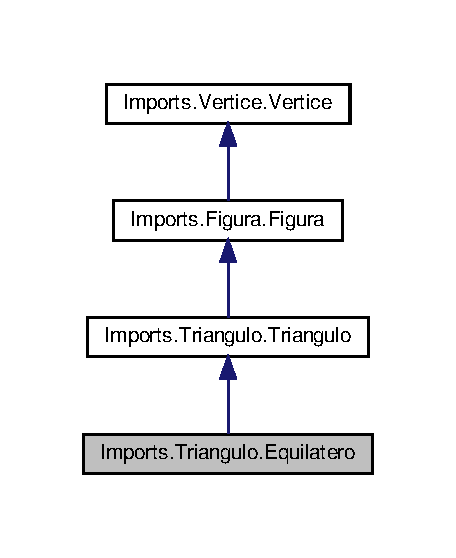
\includegraphics[width=219pt]{class_imports_1_1_triangulo_1_1_equilatero__coll__graph}
\end{center}
\end{figure}
\subsection*{Public Member Functions}
\begin{DoxyCompactItemize}
\item 
\mbox{\Hypertarget{class_imports_1_1_triangulo_1_1_equilatero_a640a63b933bc810451a37f5f5b6e9977}\label{class_imports_1_1_triangulo_1_1_equilatero_a640a63b933bc810451a37f5f5b6e9977}} 
def {\bfseries \+\_\+\+\_\+init\+\_\+\+\_\+} (self, arreglo\+Vertices, lados)
\item 
\mbox{\Hypertarget{class_imports_1_1_triangulo_1_1_equilatero_a515fef26b3975166e66bcfbd52b7b2f0}\label{class_imports_1_1_triangulo_1_1_equilatero_a515fef26b3975166e66bcfbd52b7b2f0}} 
def {\bfseries superficie} (self)
\end{DoxyCompactItemize}
\subsection*{Public Attributes}
\begin{DoxyCompactItemize}
\item 
\mbox{\Hypertarget{class_imports_1_1_triangulo_1_1_equilatero_a8ac8c9dbd59aa6842cdd686c090aee52}\label{class_imports_1_1_triangulo_1_1_equilatero_a8ac8c9dbd59aa6842cdd686c090aee52}} 
{\bfseries lista\+Vertices}
\item 
\mbox{\Hypertarget{class_imports_1_1_triangulo_1_1_equilatero_a0f2fd8d12fee7c10b42559043c6b0d74}\label{class_imports_1_1_triangulo_1_1_equilatero_a0f2fd8d12fee7c10b42559043c6b0d74}} 
{\bfseries cantidad\+Puntos}
\item 
\mbox{\Hypertarget{class_imports_1_1_triangulo_1_1_equilatero_afd547d9f5a0b18b37975c2e4d0f5dd72}\label{class_imports_1_1_triangulo_1_1_equilatero_afd547d9f5a0b18b37975c2e4d0f5dd72}} 
{\bfseries lado1}
\item 
\mbox{\Hypertarget{class_imports_1_1_triangulo_1_1_equilatero_aca1d78b3d23c2a7fb148f38a6b607b49}\label{class_imports_1_1_triangulo_1_1_equilatero_aca1d78b3d23c2a7fb148f38a6b607b49}} 
{\bfseries lado2}
\item 
\mbox{\Hypertarget{class_imports_1_1_triangulo_1_1_equilatero_a099e1644d2a182e4c632d65cbfe5d581}\label{class_imports_1_1_triangulo_1_1_equilatero_a099e1644d2a182e4c632d65cbfe5d581}} 
{\bfseries lado3}
\item 
\mbox{\Hypertarget{class_imports_1_1_triangulo_1_1_equilatero_a6be6238b62b3ca8e2016901f992941a6}\label{class_imports_1_1_triangulo_1_1_equilatero_a6be6238b62b3ca8e2016901f992941a6}} 
{\bfseries para\+Imprimir}
\item 
\mbox{\Hypertarget{class_imports_1_1_triangulo_1_1_equilatero_ac6ff67ebd27f2fa743ee4ba4df4d8ac0}\label{class_imports_1_1_triangulo_1_1_equilatero_ac6ff67ebd27f2fa743ee4ba4df4d8ac0}} 
{\bfseries area}
\item 
\mbox{\Hypertarget{class_imports_1_1_triangulo_1_1_equilatero_a57faa1ef039533e40a319df3fe7124fc}\label{class_imports_1_1_triangulo_1_1_equilatero_a57faa1ef039533e40a319df3fe7124fc}} 
{\bfseries perimetrofig}
\end{DoxyCompactItemize}


The documentation for this class was generated from the following file\+:\begin{DoxyCompactItemize}
\item 
sourcecode/\+Imports/Triangulo.\+py\end{DoxyCompactItemize}

\hypertarget{class_imports_1_1_triangulo_1_1_escaleno}{}\section{Imports.\+Triangulo.\+Escaleno Class Reference}
\label{class_imports_1_1_triangulo_1_1_escaleno}\index{Imports.\+Triangulo.\+Escaleno@{Imports.\+Triangulo.\+Escaleno}}


Inheritance diagram for Imports.\+Triangulo.\+Escaleno\+:
\nopagebreak
\begin{figure}[H]
\begin{center}
\leavevmode
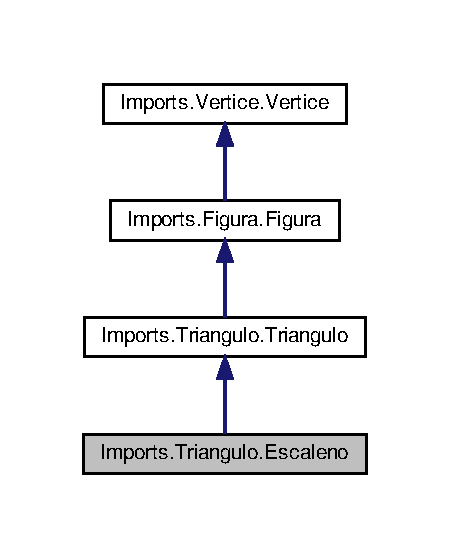
\includegraphics[width=216pt]{class_imports_1_1_triangulo_1_1_escaleno__inherit__graph}
\end{center}
\end{figure}


Collaboration diagram for Imports.\+Triangulo.\+Escaleno\+:
\nopagebreak
\begin{figure}[H]
\begin{center}
\leavevmode
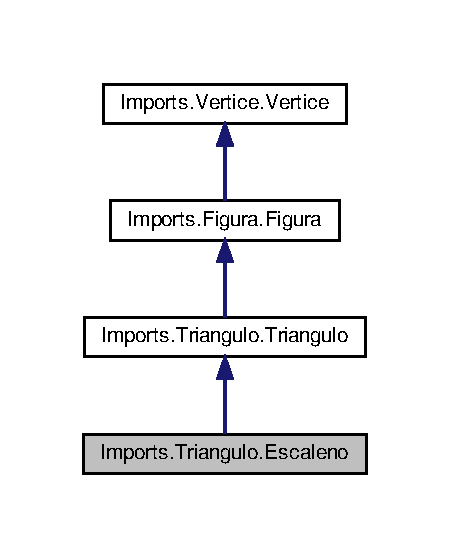
\includegraphics[width=216pt]{class_imports_1_1_triangulo_1_1_escaleno__coll__graph}
\end{center}
\end{figure}
\subsection*{Public Member Functions}
\begin{DoxyCompactItemize}
\item 
\mbox{\Hypertarget{class_imports_1_1_triangulo_1_1_escaleno_ae78d882c311580740480848b36e2b563}\label{class_imports_1_1_triangulo_1_1_escaleno_ae78d882c311580740480848b36e2b563}} 
def {\bfseries \+\_\+\+\_\+init\+\_\+\+\_\+} (self, arreglo\+Vertices, lados)
\item 
\mbox{\Hypertarget{class_imports_1_1_triangulo_1_1_escaleno_a621c4eb08304c39e70295f55cb4f5cff}\label{class_imports_1_1_triangulo_1_1_escaleno_a621c4eb08304c39e70295f55cb4f5cff}} 
def {\bfseries superficie} (self)
\end{DoxyCompactItemize}
\subsection*{Public Attributes}
\begin{DoxyCompactItemize}
\item 
\mbox{\Hypertarget{class_imports_1_1_triangulo_1_1_escaleno_a615f0a7e5feeae2b6b3d6ef5403c21b1}\label{class_imports_1_1_triangulo_1_1_escaleno_a615f0a7e5feeae2b6b3d6ef5403c21b1}} 
{\bfseries lista\+Vertices}
\item 
\mbox{\Hypertarget{class_imports_1_1_triangulo_1_1_escaleno_a3e7efd227ba7657d73d27ceb4b3c8f1b}\label{class_imports_1_1_triangulo_1_1_escaleno_a3e7efd227ba7657d73d27ceb4b3c8f1b}} 
{\bfseries cantidad\+Puntos}
\item 
\mbox{\Hypertarget{class_imports_1_1_triangulo_1_1_escaleno_ad0866a76efcc9ab7e13d1357f02f9c0e}\label{class_imports_1_1_triangulo_1_1_escaleno_ad0866a76efcc9ab7e13d1357f02f9c0e}} 
{\bfseries lado1}
\item 
\mbox{\Hypertarget{class_imports_1_1_triangulo_1_1_escaleno_aed236fc325b8b146986769f8b1dd0f78}\label{class_imports_1_1_triangulo_1_1_escaleno_aed236fc325b8b146986769f8b1dd0f78}} 
{\bfseries lado2}
\item 
\mbox{\Hypertarget{class_imports_1_1_triangulo_1_1_escaleno_a0bfe4d73af2c7d73fe19d7a415b992a6}\label{class_imports_1_1_triangulo_1_1_escaleno_a0bfe4d73af2c7d73fe19d7a415b992a6}} 
{\bfseries lado3}
\item 
\mbox{\Hypertarget{class_imports_1_1_triangulo_1_1_escaleno_a12f21275ccff3d7e1f65ef2253a15108}\label{class_imports_1_1_triangulo_1_1_escaleno_a12f21275ccff3d7e1f65ef2253a15108}} 
{\bfseries semiperimetro}
\item 
\mbox{\Hypertarget{class_imports_1_1_triangulo_1_1_escaleno_aca2f08b25c6ede79a159ab0f7bef6bfb}\label{class_imports_1_1_triangulo_1_1_escaleno_aca2f08b25c6ede79a159ab0f7bef6bfb}} 
{\bfseries para\+Imprimir}
\item 
\mbox{\Hypertarget{class_imports_1_1_triangulo_1_1_escaleno_a28d15b5d137db947fc095da608677f13}\label{class_imports_1_1_triangulo_1_1_escaleno_a28d15b5d137db947fc095da608677f13}} 
{\bfseries area}
\item 
\mbox{\Hypertarget{class_imports_1_1_triangulo_1_1_escaleno_af8c4e825edc82d6d0a7777c76b2a35fc}\label{class_imports_1_1_triangulo_1_1_escaleno_af8c4e825edc82d6d0a7777c76b2a35fc}} 
{\bfseries perimetrofig}
\end{DoxyCompactItemize}


The documentation for this class was generated from the following file\+:\begin{DoxyCompactItemize}
\item 
sourcecode/\+Imports/Triangulo.\+py\end{DoxyCompactItemize}

\hypertarget{class_imports_1_1_figura_1_1_figura}{}\section{Imports.\+Figura.\+Figura Class Reference}
\label{class_imports_1_1_figura_1_1_figura}\index{Imports.\+Figura.\+Figura@{Imports.\+Figura.\+Figura}}


Inheritance diagram for Imports.\+Figura.\+Figura\+:
\nopagebreak
\begin{figure}[H]
\begin{center}
\leavevmode
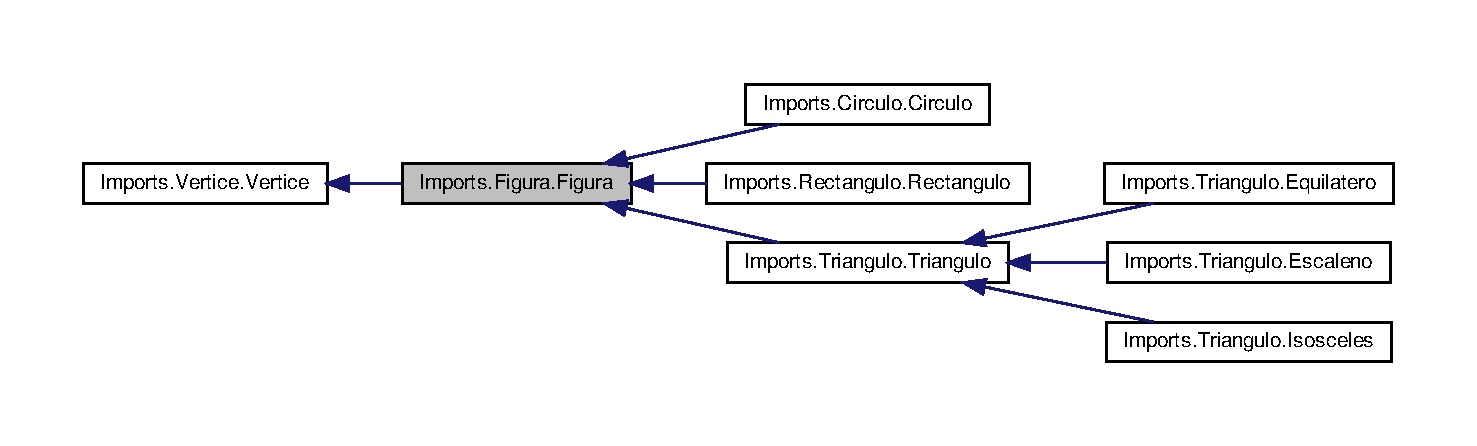
\includegraphics[width=350pt]{class_imports_1_1_figura_1_1_figura__inherit__graph}
\end{center}
\end{figure}


Collaboration diagram for Imports.\+Figura.\+Figura\+:
\nopagebreak
\begin{figure}[H]
\begin{center}
\leavevmode
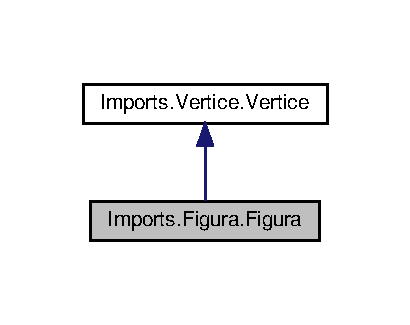
\includegraphics[width=197pt]{class_imports_1_1_figura_1_1_figura__coll__graph}
\end{center}
\end{figure}
\subsection*{Public Member Functions}
\begin{DoxyCompactItemize}
\item 
\mbox{\Hypertarget{class_imports_1_1_figura_1_1_figura_aaa458b536620df574884261aa144d183}\label{class_imports_1_1_figura_1_1_figura_aaa458b536620df574884261aa144d183}} 
def {\bfseries \+\_\+\+\_\+init\+\_\+\+\_\+} (self, vertices)
\item 
\mbox{\Hypertarget{class_imports_1_1_figura_1_1_figura_afcc51e34f169a106e916a051f0810759}\label{class_imports_1_1_figura_1_1_figura_afcc51e34f169a106e916a051f0810759}} 
def {\bfseries superficie} (self)
\item 
\mbox{\Hypertarget{class_imports_1_1_figura_1_1_figura_a8cfd4e942807c83b892f9186bdee589f}\label{class_imports_1_1_figura_1_1_figura_a8cfd4e942807c83b892f9186bdee589f}} 
def {\bfseries perimetro} (self)
\item 
\mbox{\Hypertarget{class_imports_1_1_figura_1_1_figura_a5986aa7e93785f2bb181f2cc0e20c3b2}\label{class_imports_1_1_figura_1_1_figura_a5986aa7e93785f2bb181f2cc0e20c3b2}} 
def {\bfseries \+\_\+\+\_\+invert\+\_\+\+\_\+} (self)
\end{DoxyCompactItemize}
\subsection*{Public Attributes}
\begin{DoxyCompactItemize}
\item 
\mbox{\Hypertarget{class_imports_1_1_figura_1_1_figura_add314c416e15c134067c707bf255b99a}\label{class_imports_1_1_figura_1_1_figura_add314c416e15c134067c707bf255b99a}} 
{\bfseries nombre}
\item 
\mbox{\Hypertarget{class_imports_1_1_figura_1_1_figura_a4753c4a2866bef351a81fc09a20b247a}\label{class_imports_1_1_figura_1_1_figura_a4753c4a2866bef351a81fc09a20b247a}} 
{\bfseries color}
\item 
\mbox{\Hypertarget{class_imports_1_1_figura_1_1_figura_af5c3524504133cc691658fc423c91c8d}\label{class_imports_1_1_figura_1_1_figura_af5c3524504133cc691658fc423c91c8d}} 
{\bfseries para\+Imprimir}
\item 
\mbox{\Hypertarget{class_imports_1_1_figura_1_1_figura_a645cf8d8d74cbefbb3e4abe82990f173}\label{class_imports_1_1_figura_1_1_figura_a645cf8d8d74cbefbb3e4abe82990f173}} 
{\bfseries identificador}
\item 
\mbox{\Hypertarget{class_imports_1_1_figura_1_1_figura_aec730795d9bb7daee9fd62521c2e0236}\label{class_imports_1_1_figura_1_1_figura_aec730795d9bb7daee9fd62521c2e0236}} 
{\bfseries auto\+Incrementado}
\item 
\mbox{\Hypertarget{class_imports_1_1_figura_1_1_figura_a1a045513cb4f6b45122ae94085418817}\label{class_imports_1_1_figura_1_1_figura_a1a045513cb4f6b45122ae94085418817}} 
{\bfseries lista\+Vertices}
\item 
\mbox{\Hypertarget{class_imports_1_1_figura_1_1_figura_a954959dd00d56582db4c5b40336089df}\label{class_imports_1_1_figura_1_1_figura_a954959dd00d56582db4c5b40336089df}} 
{\bfseries lado}
\item 
\mbox{\Hypertarget{class_imports_1_1_figura_1_1_figura_af8859e344f1e43aa6124d167d821a3b5}\label{class_imports_1_1_figura_1_1_figura_af8859e344f1e43aa6124d167d821a3b5}} 
{\bfseries area}
\item 
\mbox{\Hypertarget{class_imports_1_1_figura_1_1_figura_ab7b5a1a11f492e83207695daf37b1418}\label{class_imports_1_1_figura_1_1_figura_ab7b5a1a11f492e83207695daf37b1418}} 
{\bfseries perimetrofig}
\item 
\mbox{\Hypertarget{class_imports_1_1_figura_1_1_figura_a08b1b4efe89a1729df093407db6739b1}\label{class_imports_1_1_figura_1_1_figura_a08b1b4efe89a1729df093407db6739b1}} 
{\bfseries cantidad\+Puntos}
\end{DoxyCompactItemize}


The documentation for this class was generated from the following file\+:\begin{DoxyCompactItemize}
\item 
sourcecode/\+Imports/Figura.\+py\end{DoxyCompactItemize}

\hypertarget{class_imports_1_1_impresora_1_1_impresora}{}\section{Imports.\+Impresora.\+Impresora Class Reference}
\label{class_imports_1_1_impresora_1_1_impresora}\index{Imports.\+Impresora.\+Impresora@{Imports.\+Impresora.\+Impresora}}
\subsection*{Public Member Functions}
\begin{DoxyCompactItemize}
\item 
\mbox{\Hypertarget{class_imports_1_1_impresora_1_1_impresora_acb8b9c99498daef1583b6de79ae200f2}\label{class_imports_1_1_impresora_1_1_impresora_acb8b9c99498daef1583b6de79ae200f2}} 
def {\bfseries \+\_\+\+\_\+init\+\_\+\+\_\+} (self, figura)
\item 
\mbox{\Hypertarget{class_imports_1_1_impresora_1_1_impresora_aae9abb46f5f8829b6ca09ca75f7c1de3}\label{class_imports_1_1_impresora_1_1_impresora_aae9abb46f5f8829b6ca09ca75f7c1de3}} 
def {\bfseries imprimir\+Pantalla} (self, figura)
\item 
\mbox{\Hypertarget{class_imports_1_1_impresora_1_1_impresora_af806c391a24ab629fa25764c4c840f08}\label{class_imports_1_1_impresora_1_1_impresora_af806c391a24ab629fa25764c4c840f08}} 
def {\bfseries imprimir\+Archivo} (self, objeto)
\end{DoxyCompactItemize}


The documentation for this class was generated from the following file\+:\begin{DoxyCompactItemize}
\item 
sourcecode/\+Imports/Impresora.\+py\end{DoxyCompactItemize}

\hypertarget{class_imports_1_1_triangulo_1_1_isosceles}{}\section{Imports.\+Triangulo.\+Isosceles Class Reference}
\label{class_imports_1_1_triangulo_1_1_isosceles}\index{Imports.\+Triangulo.\+Isosceles@{Imports.\+Triangulo.\+Isosceles}}


Inheritance diagram for Imports.\+Triangulo.\+Isosceles\+:
\nopagebreak
\begin{figure}[H]
\begin{center}
\leavevmode
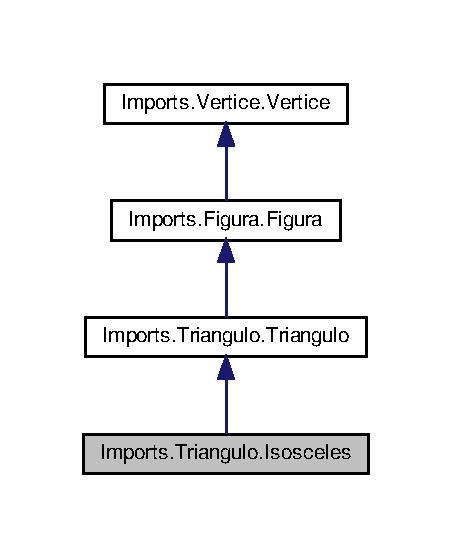
\includegraphics[width=217pt]{class_imports_1_1_triangulo_1_1_isosceles__inherit__graph}
\end{center}
\end{figure}


Collaboration diagram for Imports.\+Triangulo.\+Isosceles\+:
\nopagebreak
\begin{figure}[H]
\begin{center}
\leavevmode
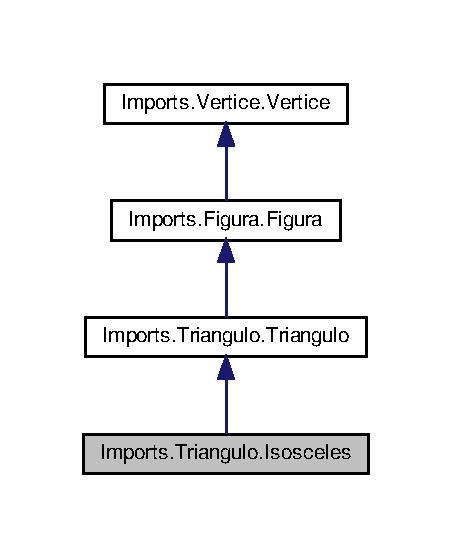
\includegraphics[width=217pt]{class_imports_1_1_triangulo_1_1_isosceles__coll__graph}
\end{center}
\end{figure}
\subsection*{Public Member Functions}
\begin{DoxyCompactItemize}
\item 
\mbox{\Hypertarget{class_imports_1_1_triangulo_1_1_isosceles_a379ba78e7432042a35e2036617606a04}\label{class_imports_1_1_triangulo_1_1_isosceles_a379ba78e7432042a35e2036617606a04}} 
def {\bfseries \+\_\+\+\_\+init\+\_\+\+\_\+} (self, arreglo\+Vertices, lados)
\item 
\mbox{\Hypertarget{class_imports_1_1_triangulo_1_1_isosceles_a02b6af8b983c6c3c4e9a567aa29981b4}\label{class_imports_1_1_triangulo_1_1_isosceles_a02b6af8b983c6c3c4e9a567aa29981b4}} 
def {\bfseries superficie} (self)
\end{DoxyCompactItemize}
\subsection*{Public Attributes}
\begin{DoxyCompactItemize}
\item 
\mbox{\Hypertarget{class_imports_1_1_triangulo_1_1_isosceles_a8a9aab1533dcf3483649f0db6636bcd3}\label{class_imports_1_1_triangulo_1_1_isosceles_a8a9aab1533dcf3483649f0db6636bcd3}} 
{\bfseries lista\+Vertices}
\item 
\mbox{\Hypertarget{class_imports_1_1_triangulo_1_1_isosceles_a54f9c0d8939caf0bb174de363ac8745e}\label{class_imports_1_1_triangulo_1_1_isosceles_a54f9c0d8939caf0bb174de363ac8745e}} 
{\bfseries cantidad\+Puntos}
\item 
\mbox{\Hypertarget{class_imports_1_1_triangulo_1_1_isosceles_a6ebf7f4fc4d60621f7fc219012e40760}\label{class_imports_1_1_triangulo_1_1_isosceles_a6ebf7f4fc4d60621f7fc219012e40760}} 
{\bfseries distancias}
\item 
\mbox{\Hypertarget{class_imports_1_1_triangulo_1_1_isosceles_a4a7019dd65660263ce8735d6fe7b6841}\label{class_imports_1_1_triangulo_1_1_isosceles_a4a7019dd65660263ce8735d6fe7b6841}} 
{\bfseries lado1}
\item 
\mbox{\Hypertarget{class_imports_1_1_triangulo_1_1_isosceles_aef381f47d39f184278eaf6fd88bda9d5}\label{class_imports_1_1_triangulo_1_1_isosceles_aef381f47d39f184278eaf6fd88bda9d5}} 
{\bfseries lado2}
\item 
\mbox{\Hypertarget{class_imports_1_1_triangulo_1_1_isosceles_aaa6364106c10ec27b30c47a0e666b5c9}\label{class_imports_1_1_triangulo_1_1_isosceles_aaa6364106c10ec27b30c47a0e666b5c9}} 
{\bfseries lado3}
\item 
\mbox{\Hypertarget{class_imports_1_1_triangulo_1_1_isosceles_a502f7d5f22f8bf7fd75b4b51a04189e3}\label{class_imports_1_1_triangulo_1_1_isosceles_a502f7d5f22f8bf7fd75b4b51a04189e3}} 
{\bfseries para\+Imprimir}
\item 
\mbox{\Hypertarget{class_imports_1_1_triangulo_1_1_isosceles_a18f8fac309febc4afc96f28b9942443a}\label{class_imports_1_1_triangulo_1_1_isosceles_a18f8fac309febc4afc96f28b9942443a}} 
{\bfseries area}
\item 
\mbox{\Hypertarget{class_imports_1_1_triangulo_1_1_isosceles_a7595594cc4effb00a77a2990e39771a2}\label{class_imports_1_1_triangulo_1_1_isosceles_a7595594cc4effb00a77a2990e39771a2}} 
{\bfseries perimetrofig}
\end{DoxyCompactItemize}


The documentation for this class was generated from the following file\+:\begin{DoxyCompactItemize}
\item 
sourcecode/\+Imports/Triangulo.\+py\end{DoxyCompactItemize}

\hypertarget{class_imports_1_1_principal_1_1_principal}{}\section{Imports.\+Principal.\+Principal Class Reference}
\label{class_imports_1_1_principal_1_1_principal}\index{Imports.\+Principal.\+Principal@{Imports.\+Principal.\+Principal}}
\subsection*{Public Member Functions}
\begin{DoxyCompactItemize}
\item 
\mbox{\Hypertarget{class_imports_1_1_principal_1_1_principal_ab4584824e61de88e435c8a6db58e81fc}\label{class_imports_1_1_principal_1_1_principal_ab4584824e61de88e435c8a6db58e81fc}} 
def {\bfseries \+\_\+\+\_\+init\+\_\+\+\_\+} (self)
\item 
\mbox{\Hypertarget{class_imports_1_1_principal_1_1_principal_acc3ab870d562121bfc230c2709678aba}\label{class_imports_1_1_principal_1_1_principal_acc3ab870d562121bfc230c2709678aba}} 
def {\bfseries menu} (self)
\item 
\mbox{\Hypertarget{class_imports_1_1_principal_1_1_principal_a423de8f65aa9bce0b30dc3eb4db5e1e6}\label{class_imports_1_1_principal_1_1_principal_a423de8f65aa9bce0b30dc3eb4db5e1e6}} 
def {\bfseries opcion} (self)
\item 
\mbox{\Hypertarget{class_imports_1_1_principal_1_1_principal_ada9da089d294a780fdc84c2db554f40c}\label{class_imports_1_1_principal_1_1_principal_ada9da089d294a780fdc84c2db554f40c}} 
def {\bfseries Hacer\+Arreglo\+Vertices} (self, cantidad)
\item 
\mbox{\Hypertarget{class_imports_1_1_principal_1_1_principal_a29cb7674a3fc313a0b46480d1977c1d7}\label{class_imports_1_1_principal_1_1_principal_a29cb7674a3fc313a0b46480d1977c1d7}} 
def {\bfseries M\+T\+D\+R\+E\+C\+T\+A\+N\+G\+U\+LO} (self)
\item 
\mbox{\Hypertarget{class_imports_1_1_principal_1_1_principal_a440ccddd30dd46474b98c13b9127dfa2}\label{class_imports_1_1_principal_1_1_principal_a440ccddd30dd46474b98c13b9127dfa2}} 
def {\bfseries M\+T\+D\+C\+I\+R\+C\+U\+LO} (self)
\item 
\mbox{\Hypertarget{class_imports_1_1_principal_1_1_principal_ac5779377f4762c9493d9b746436694cf}\label{class_imports_1_1_principal_1_1_principal_ac5779377f4762c9493d9b746436694cf}} 
def {\bfseries M\+T\+D\+T\+R\+I\+A\+N\+G\+U\+LO} (self)
\end{DoxyCompactItemize}
\subsection*{Public Attributes}
\begin{DoxyCompactItemize}
\item 
\mbox{\Hypertarget{class_imports_1_1_principal_1_1_principal_a26f556fca3f8707beb54319846e9270f}\label{class_imports_1_1_principal_1_1_principal_a26f556fca3f8707beb54319846e9270f}} 
{\bfseries entrada}
\item 
\mbox{\Hypertarget{class_imports_1_1_principal_1_1_principal_ac611e07a1a4bccd593c7412d8f23a6d2}\label{class_imports_1_1_principal_1_1_principal_ac611e07a1a4bccd593c7412d8f23a6d2}} 
{\bfseries arreglo\+Vertices}
\item 
\mbox{\Hypertarget{class_imports_1_1_principal_1_1_principal_ab42455f4dc6c24a21bcd849a6ca01f49}\label{class_imports_1_1_principal_1_1_principal_ab42455f4dc6c24a21bcd849a6ca01f49}} 
{\bfseries distancias}
\end{DoxyCompactItemize}


The documentation for this class was generated from the following file\+:\begin{DoxyCompactItemize}
\item 
sourcecode/\+Imports/Principal.\+py\end{DoxyCompactItemize}

\hypertarget{class_imports_1_1_rectangulo_1_1_rectangulo}{}\section{Imports.\+Rectangulo.\+Rectangulo Class Reference}
\label{class_imports_1_1_rectangulo_1_1_rectangulo}\index{Imports.\+Rectangulo.\+Rectangulo@{Imports.\+Rectangulo.\+Rectangulo}}


Inheritance diagram for Imports.\+Rectangulo.\+Rectangulo\+:
\nopagebreak
\begin{figure}[H]
\begin{center}
\leavevmode
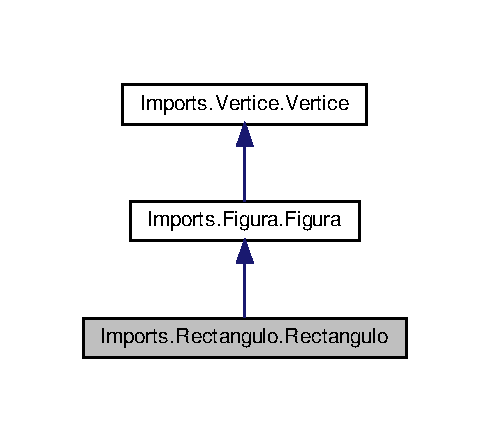
\includegraphics[width=235pt]{class_imports_1_1_rectangulo_1_1_rectangulo__inherit__graph}
\end{center}
\end{figure}


Collaboration diagram for Imports.\+Rectangulo.\+Rectangulo\+:
\nopagebreak
\begin{figure}[H]
\begin{center}
\leavevmode
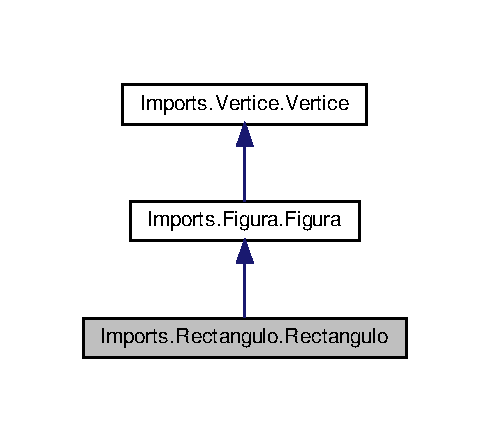
\includegraphics[width=235pt]{class_imports_1_1_rectangulo_1_1_rectangulo__coll__graph}
\end{center}
\end{figure}
\subsection*{Public Member Functions}
\begin{DoxyCompactItemize}
\item 
\mbox{\Hypertarget{class_imports_1_1_rectangulo_1_1_rectangulo_aa6ab5baaedcd4a9c6fb090814cde383b}\label{class_imports_1_1_rectangulo_1_1_rectangulo_aa6ab5baaedcd4a9c6fb090814cde383b}} 
def {\bfseries \+\_\+\+\_\+init\+\_\+\+\_\+} (self, arreglo\+Vertices)
\item 
\mbox{\Hypertarget{class_imports_1_1_rectangulo_1_1_rectangulo_a5b7f4096dc85ee69031961b350c18246}\label{class_imports_1_1_rectangulo_1_1_rectangulo_a5b7f4096dc85ee69031961b350c18246}} 
def {\bfseries superficie} (self)
\item 
\mbox{\Hypertarget{class_imports_1_1_rectangulo_1_1_rectangulo_a0ae19a4ba2f6832f66a0fdd898e3157c}\label{class_imports_1_1_rectangulo_1_1_rectangulo_a0ae19a4ba2f6832f66a0fdd898e3157c}} 
def {\bfseries perimetro} (self)
\end{DoxyCompactItemize}
\subsection*{Public Attributes}
\begin{DoxyCompactItemize}
\item 
\mbox{\Hypertarget{class_imports_1_1_rectangulo_1_1_rectangulo_a36ca6e796e1f7b657c571e98547537e3}\label{class_imports_1_1_rectangulo_1_1_rectangulo_a36ca6e796e1f7b657c571e98547537e3}} 
{\bfseries base}
\item 
\mbox{\Hypertarget{class_imports_1_1_rectangulo_1_1_rectangulo_a15404135d90de586e52e83075d74c1e8}\label{class_imports_1_1_rectangulo_1_1_rectangulo_a15404135d90de586e52e83075d74c1e8}} 
{\bfseries altura}
\item 
\mbox{\Hypertarget{class_imports_1_1_rectangulo_1_1_rectangulo_abebc186ecfd1eba7524ff4e785f24ac5}\label{class_imports_1_1_rectangulo_1_1_rectangulo_abebc186ecfd1eba7524ff4e785f24ac5}} 
{\bfseries cantidad\+Puntos}
\item 
\mbox{\Hypertarget{class_imports_1_1_rectangulo_1_1_rectangulo_abfc7b38112507df38e844f7193280ffe}\label{class_imports_1_1_rectangulo_1_1_rectangulo_abfc7b38112507df38e844f7193280ffe}} 
{\bfseries lista\+Vertices}
\item 
\mbox{\Hypertarget{class_imports_1_1_rectangulo_1_1_rectangulo_aed720603f3b0477a0e5f65f8640dfea1}\label{class_imports_1_1_rectangulo_1_1_rectangulo_aed720603f3b0477a0e5f65f8640dfea1}} 
{\bfseries para\+Imprimir}
\item 
\mbox{\Hypertarget{class_imports_1_1_rectangulo_1_1_rectangulo_abecb88c5bdf7b9a3ae65051c532f4c1f}\label{class_imports_1_1_rectangulo_1_1_rectangulo_abecb88c5bdf7b9a3ae65051c532f4c1f}} 
{\bfseries area}
\item 
\mbox{\Hypertarget{class_imports_1_1_rectangulo_1_1_rectangulo_a551ae87f2231e75d52de16e0239bcde0}\label{class_imports_1_1_rectangulo_1_1_rectangulo_a551ae87f2231e75d52de16e0239bcde0}} 
{\bfseries perimetrofig}
\end{DoxyCompactItemize}


The documentation for this class was generated from the following file\+:\begin{DoxyCompactItemize}
\item 
sourcecode/\+Imports/Rectangulo.\+py\end{DoxyCompactItemize}

\hypertarget{class_imports_1_1_triangulo_1_1_triangulo}{}\section{Imports.\+Triangulo.\+Triangulo Class Reference}
\label{class_imports_1_1_triangulo_1_1_triangulo}\index{Imports.\+Triangulo.\+Triangulo@{Imports.\+Triangulo.\+Triangulo}}


Inheritance diagram for Imports.\+Triangulo.\+Triangulo\+:
\nopagebreak
\begin{figure}[H]
\begin{center}
\leavevmode
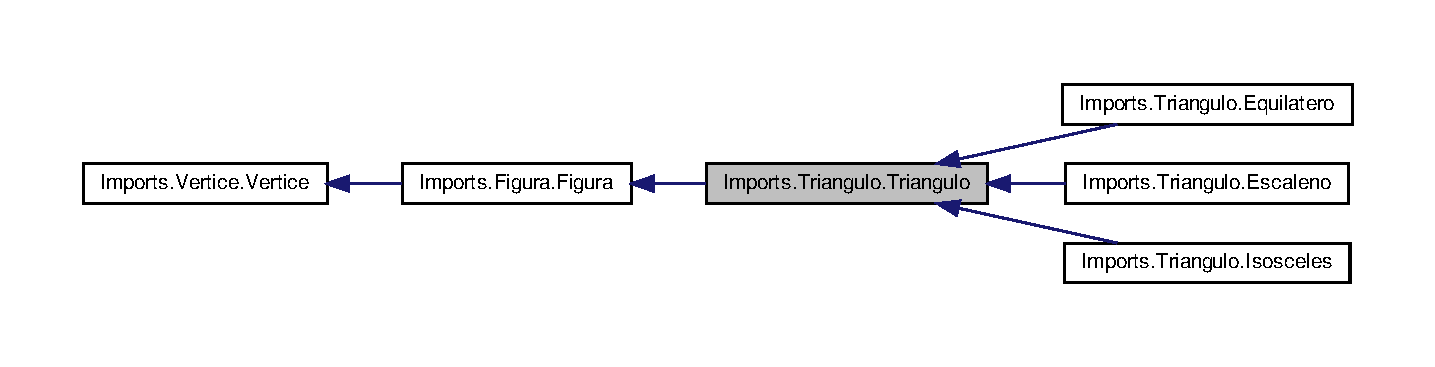
\includegraphics[width=350pt]{class_imports_1_1_triangulo_1_1_triangulo__inherit__graph}
\end{center}
\end{figure}


Collaboration diagram for Imports.\+Triangulo.\+Triangulo\+:
\nopagebreak
\begin{figure}[H]
\begin{center}
\leavevmode
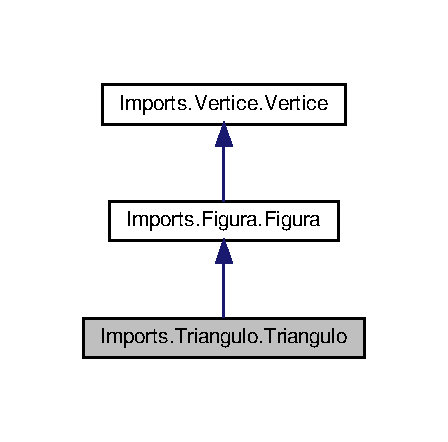
\includegraphics[width=215pt]{class_imports_1_1_triangulo_1_1_triangulo__coll__graph}
\end{center}
\end{figure}
\subsection*{Public Member Functions}
\begin{DoxyCompactItemize}
\item 
\mbox{\Hypertarget{class_imports_1_1_triangulo_1_1_triangulo_aca2395c6ea6b671b4d1f809e6ca4614a}\label{class_imports_1_1_triangulo_1_1_triangulo_aca2395c6ea6b671b4d1f809e6ca4614a}} 
def {\bfseries \+\_\+\+\_\+init\+\_\+\+\_\+} (self)
\item 
\mbox{\Hypertarget{class_imports_1_1_triangulo_1_1_triangulo_a45012d511c1137466dc9dc9138f111d6}\label{class_imports_1_1_triangulo_1_1_triangulo_a45012d511c1137466dc9dc9138f111d6}} 
def {\bfseries perimetro} (self)
\end{DoxyCompactItemize}
\subsection*{Public Attributes}
\begin{DoxyCompactItemize}
\item 
\mbox{\Hypertarget{class_imports_1_1_triangulo_1_1_triangulo_a88d5d8832e37e9543881a7370d28dc81}\label{class_imports_1_1_triangulo_1_1_triangulo_a88d5d8832e37e9543881a7370d28dc81}} 
{\bfseries lado1}
\item 
\mbox{\Hypertarget{class_imports_1_1_triangulo_1_1_triangulo_abb9022ca4d70bbc86fadd202e4479d96}\label{class_imports_1_1_triangulo_1_1_triangulo_abb9022ca4d70bbc86fadd202e4479d96}} 
{\bfseries lado2}
\item 
\mbox{\Hypertarget{class_imports_1_1_triangulo_1_1_triangulo_a27922fe444d0737e0b99bacb1970760a}\label{class_imports_1_1_triangulo_1_1_triangulo_a27922fe444d0737e0b99bacb1970760a}} 
{\bfseries lado3}
\end{DoxyCompactItemize}


The documentation for this class was generated from the following file\+:\begin{DoxyCompactItemize}
\item 
sourcecode/\+Imports/Triangulo.\+py\end{DoxyCompactItemize}

\hypertarget{class_imports_1_1_vertice_1_1_vertice}{}\section{Imports.\+Vertice.\+Vertice Class Reference}
\label{class_imports_1_1_vertice_1_1_vertice}\index{Imports.\+Vertice.\+Vertice@{Imports.\+Vertice.\+Vertice}}


Inheritance diagram for Imports.\+Vertice.\+Vertice\+:
\nopagebreak
\begin{figure}[H]
\begin{center}
\leavevmode
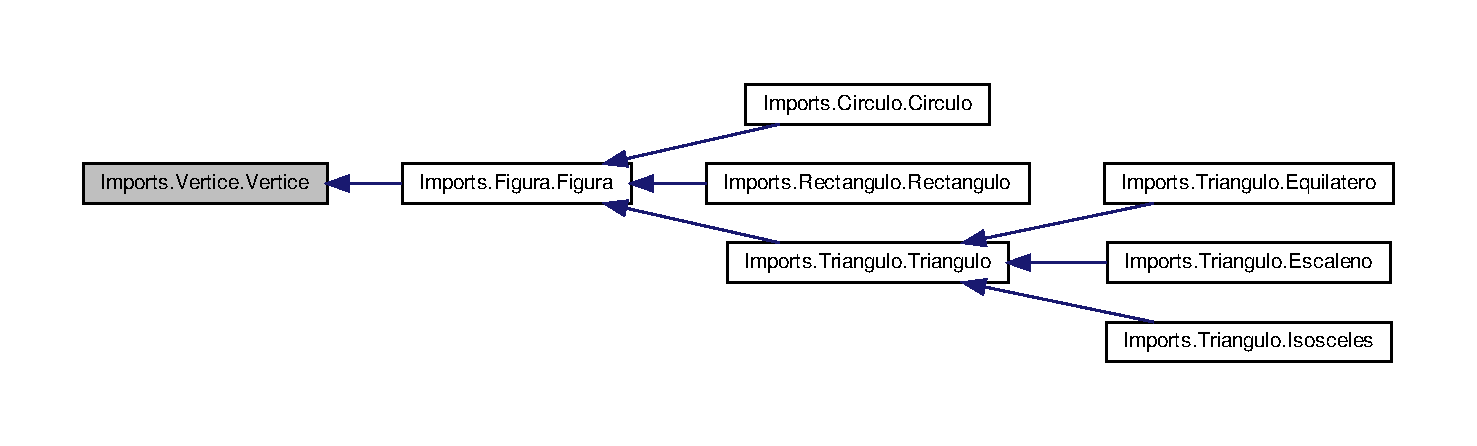
\includegraphics[width=350pt]{class_imports_1_1_vertice_1_1_vertice__inherit__graph}
\end{center}
\end{figure}
\subsection*{Public Member Functions}
\begin{DoxyCompactItemize}
\item 
\mbox{\Hypertarget{class_imports_1_1_vertice_1_1_vertice_a8b8a76f8adcbf78de00db07756c8d976}\label{class_imports_1_1_vertice_1_1_vertice_a8b8a76f8adcbf78de00db07756c8d976}} 
def {\bfseries \+\_\+\+\_\+init\+\_\+\+\_\+} (self)
\item 
\mbox{\Hypertarget{class_imports_1_1_vertice_1_1_vertice_af62a2375ac42f08969130c96d3466edf}\label{class_imports_1_1_vertice_1_1_vertice_af62a2375ac42f08969130c96d3466edf}} 
def {\bfseries \+\_\+\+\_\+rshift\+\_\+\+\_\+} (self, other)
\item 
\mbox{\Hypertarget{class_imports_1_1_vertice_1_1_vertice_a8ddbbc9c3b7b9a6454ed39d30e7e19c9}\label{class_imports_1_1_vertice_1_1_vertice_a8ddbbc9c3b7b9a6454ed39d30e7e19c9}} 
def {\bfseries \+\_\+\+\_\+invert\+\_\+\+\_\+} (self)
\end{DoxyCompactItemize}
\subsection*{Public Attributes}
\begin{DoxyCompactItemize}
\item 
\mbox{\Hypertarget{class_imports_1_1_vertice_1_1_vertice_aef1b3062fd8276e1d16b12ffda47494b}\label{class_imports_1_1_vertice_1_1_vertice_aef1b3062fd8276e1d16b12ffda47494b}} 
{\bfseries x}
\item 
\mbox{\Hypertarget{class_imports_1_1_vertice_1_1_vertice_af85eb9467fc87af9dba7b37e60387a1a}\label{class_imports_1_1_vertice_1_1_vertice_af85eb9467fc87af9dba7b37e60387a1a}} 
{\bfseries y}
\item 
\mbox{\Hypertarget{class_imports_1_1_vertice_1_1_vertice_ac78741bd9dca11609db7fd7ac2fffaf2}\label{class_imports_1_1_vertice_1_1_vertice_ac78741bd9dca11609db7fd7ac2fffaf2}} 
{\bfseries identificador}
\end{DoxyCompactItemize}


The documentation for this class was generated from the following file\+:\begin{DoxyCompactItemize}
\item 
sourcecode/\+Imports/Vertice.\+py\end{DoxyCompactItemize}

%--- End generated contents ---

% Index
\backmatter
\newpage
\phantomsection
\clearemptydoublepage
\addcontentsline{toc}{chapter}{Index}
\printindex

\end{document}
